% Chapter Template

\chapter{State of the Art} % Main chapter title

\label{Chapter3} % Change X to a consecutive number; for referencing this chapter elsewhere, use \ref{ChapterX}


\section{Introduction}

TODO, be a *neutral* presentation of the current state of this technology. Give a big information dump to the reader.


\section{Commercial Smartcubes}

Commercial Smartcubes are special Rubik's Cubes built around sensors that can detect face turns and transmit that information over Bluetooth.
Some models can also measure and transmit data about the cube's orientation.

At the time of writing, there are four major smartcubes on the market: the Giiker Cube, the Go Cube, the Rubik's Connected (which is powered by GoCube technology) and the Gans 356i.
This section will discuss the internal components of each of these cubes that provide this move-tracking functionality.

\subsection{Giiker Cube}
The Xiaomi Giiker Cube was released in September 2018 making it the first commercial smartcube on the market \cite{giiker-thecubicle}.
This "Supercube" as it was branded, used a relatively simple system for tracking the cube's movements.
The core of the cube is built around a small circuit board with a microcontroller that measures the cube's movements and a bluetooth antenna that transmits those moves wirelessly (Figure ~\ref{fig:giiker-internal-board}).
The microcontroller detects each face turn by reading the voltage drop across a small circuit embedded within each center cap (Figure ~\ref{fig:giiker-center-front}).
The center cap circuit controls its output voltage by using a copper brush to change between four separate electric paths, three different resistors and ground, as each face rotates (Figure ~\ref{fig:giiker-center-brush}). \cite{giiker-internals}


% How to do a sub-figure: https://tex.stackexchange.com/a/37597
\begin{figure}
    \centering
    \begin{subfigure}{0.25\textwidth}
        \centering
        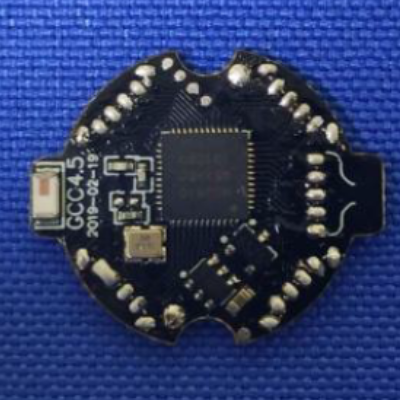
\includegraphics[width=.90\linewidth]{Figures/3 State of the Art/giiker-internal-board.png}
        \caption{Internal Board \cite{giiker-internals}}
        \label{fig:giiker-internal-board}
    \end{subfigure}%
    \begin{subfigure}{0.25\textwidth}
        \centering
        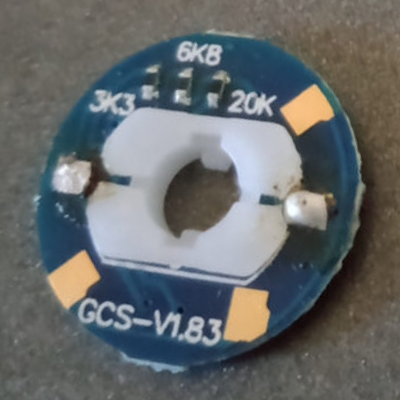
\includegraphics[width=.90\linewidth]{Figures/3 State of the Art/giiker-center-front.png}
        \caption{Center Cap Board \cite{eggins-giiker-internals}}
        \label{fig:giiker-center-front}
    \end{subfigure}%
    \begin{subfigure}{0.25\textwidth}
        \centering
        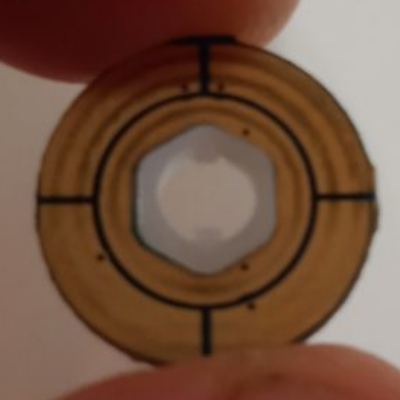
\includegraphics[width=.90\linewidth]{Figures/3 State of the Art/giiker-center-pads.png}
        \caption{Center Cap Pads \cite{eggins-giiker-internals}}
        \label{fig:giiker-center-pads}
    \end{subfigure}%
    \begin{subfigure}{0.25\textwidth}
        \centering
        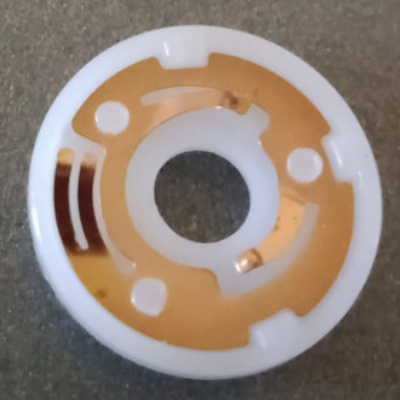
\includegraphics[width=.90\linewidth]{Figures/3 State of the Art/giiker-center-brush.png}
        \caption{Center Cap Brush \cite{eggins-giiker-internals}}
        \label{fig:giiker-center-brush}
    \end{subfigure}%
    \caption{The internal components of the Giiker Cube}
    \label{fig:giiker-internal-components}
\end{figure}

\subsection{Go Cube}
Announced on Kickstarter in June 2018, Patricula's GoCube was the first smartcube to include a gyroscope that would track a Rubik's Cube's orientation in addition to the face turns applied to it. \cite{gocube-product-launch-video}
Like the Giiker Cube before it, the GoCube's core contains a small circuit board with the main electronics including a microcontroller, bluetooth antenna, and the added gyroscope (Figure ~\ref{fig:gocube-core}). 
Though the teardown pictures from the Go Cube's FCC filing aren't particularly clear, it appears that the cube registers face turns similarly to the Giiker Cube: by producing a voltage drop via changing which one of the four resistors shown across the bottom of the center cap board in Figure ~\ref{fig:gocube-cap-chip} is in series with the circuit.

GoCube also serves as the underlying technology for the Rubik's Connected, the official smartcube from The Rubik's Company. \cite{gocube-rubiksconnected}

% How to do a sub-figure: https://tex.stackexchange.com/a/37597
\begin{figure}
    \centering
    \begin{subfigure}{0.25\textwidth}
        \centering
        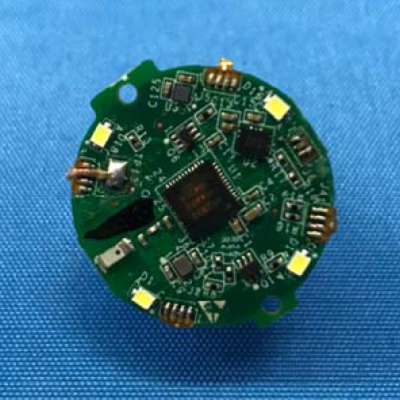
\includegraphics[width=.90\linewidth]{Figures/3 State of the Art/gocube-core.png}
        \caption{Internal Board}
        \label{fig:gocube-core}
    \end{subfigure}%
    \begin{subfigure}{0.25\textwidth}
        \centering
        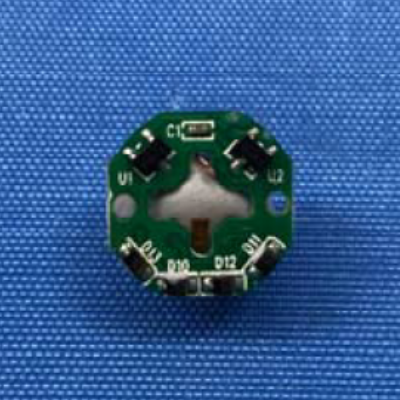
\includegraphics[width=.90\linewidth]{Figures/3 State of the Art/gocube-cap-chip.png}
        \caption{Center Cap Board}
        \label{fig:gocube-cap-chip}
    \end{subfigure}%
    \begin{subfigure}{0.50\textwidth}
        \centering
        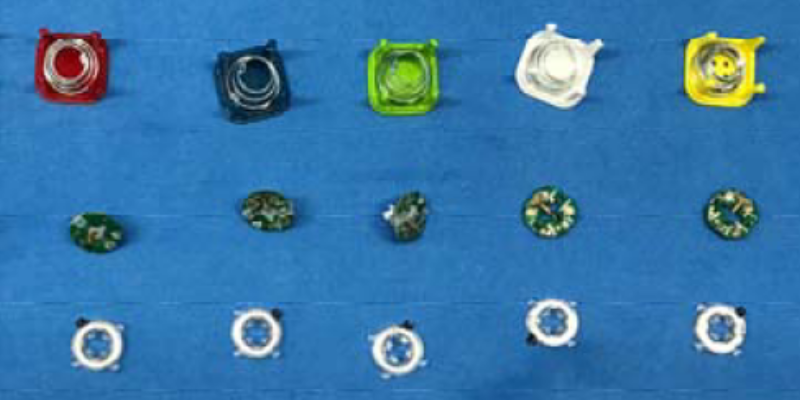
\includegraphics[width=.90\linewidth]{Figures/3 State of the Art/gocube-centers.png}
        \caption{Full Center Cap Teardown}
        \label{fig:gocube-centers}
    \end{subfigure}%
    \caption{The internal components of the Go Cube \cite{gocube-internals}}
    \label{fig:gocube-internal-components}
\end{figure}

\subsection{Gans 356i}
Released in July 2019, the Gans 356i was the first commercial smartcube produced by a traditional speedcube manufacturer. \cite{gans356i-thecubicle}
While the Gans 356i also uses a microcontroller to process the face turns and Bluetooth to transmit the move data, it tracks moves not through changing resistors in and out of a circuit, but via six plastic rods that connect the outer center caps to internal rotary encoders (Figure ~\ref{fig:gans356i-core}).

\begin{figure}
    \centering
    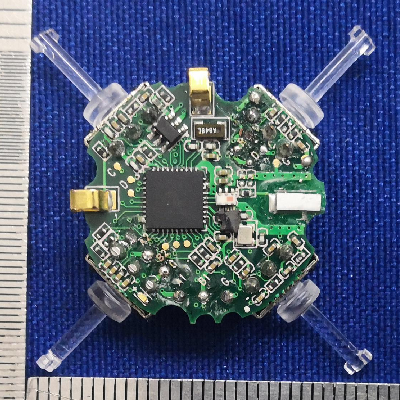
\includegraphics{Figures/3 State of the Art/gans356i-core.png}
    \decoRule
    \caption[Gans 356i Teardown]{The Gans 356i Cube's internal components. \cite{gans-356i-internals}}
    \label{fig:gans356i-core}
\end{figure}


\section{Academia}
In addition to the various commercial smartcubes, many academic research projects have involved some element of tracking the state/face turns of a Rubik's Cube.

This section summarizes the current state of academic research into using computer vision, magnetic resonance, and a muscle-tracking armband to track the state of a Rubik's Cube.


\subsection{Computer Vision}
\label{subsec:computer-vision}
Computer Vision refers to the "field of Artificial Intelligence (AI) that enables computers and systems to derive meaningful information from digital images, videos, and other visual inputs." \cite{ibm-cv-definition}
Since human manipulation of a Rubik's Cube is a physical, observable process, Computer Vision algorithms could be developed to extract face turn information from videos of Rubik's Cube solutions.

This section summarizes some of the relevant research in this area, including computer vision algorithms capable of extracting individual sticker colors from video, measuring the angle of rotation of a specific face, and detection of entire face turns and face turn sequences.

\subsubsection{Sticker Color Classification}
In 2015, Jay Hack, an graduate student studying Computer Science at Stanford developed a neural network capable of recognizing the colors of a Rubik's Cube face from video in various lighting conditions.
His algorithm could classify frames within 7 milliseconds with 92\% accuracy. \cite{hackrubik}

\subsubsection{Measuring a Face's Angle of Rotation}
In 2019, OpenAI et al. published a viral video of a robot hand that had taught itself to solve a Rubik's Cube.
While the final, most successful version of the robot hand's software used a Giiker Cube to obtain the current rotational state of the cube, OpenAI et al. also researched the viability of tracking a Rubik's Cube's position using only computer vision.
Their most successful vision-only algorithm measured only the rotation angle of the top-most face on the Rubik's Cube and assumed significant hardware requirements: a modified sticker set for the Rubik's Cube, a well-lit environment, three strategically positioned RBG Basler cameras, and a neural network trained on "a pool of optimizer nodes, each of which uses 8 NVIDIA V100 GPUs and 64 CPU cores".
At peak performance, their vision-only algorithm's average error (the difference between the predicted face angle and the actual face angle) was 15.92$^\circ$, nearly three times the 5.90$^\circ$ average error of the hardware-based face angle measurement. \cite{openai2019rubiks}

\subsubsection{Classification of Single Moves and Entire Move Sequences}
In 2020, Junshen Kevin Chen, Wanze Xie, and Zhouheng Sun, graduate Computer Science students at Stanford created the DeepCube dataset consisting of over 20,000 videos of Rubik's Cube face turns with consistent lighting and backgrounds. 
They also built a neural network to classify the videos with the face turn they contained.
Their best performing model only made "one mistake every 15 moves" which corresponds to a 93.3\% accuracy. \cite{chendeepcube}


\subsection{Magnetic Resonance}
In 2018, Maria Mannone et al. used the IM3D magnetic 3D motion tracking technology introduced by Huang et al. \cite{im3d} to track the state of a Rubik's Cube across various movements for the purpose of generating a sequence of musical chords.
This approach to turn tracking requires a special array of magnetic coils as shown in Figure ~\ref{fig:im3d-architecture} and the installation of "multiple small, light-
weight, wireless markers (LC coils) with unique IDs" (a process that requires permanant modifications to the cube as evidenced by the damaged plastic in Figure ~\ref{fig:cubeharmonic-trackers}).
Mannone et al. reported no issues with mistakes in the move tracking technology.

% How to do a sub-figure: https://tex.stackexchange.com/a/37597
\begin{figure}
    \centering
    \begin{subfigure}{0.60\textwidth}
        \centering
        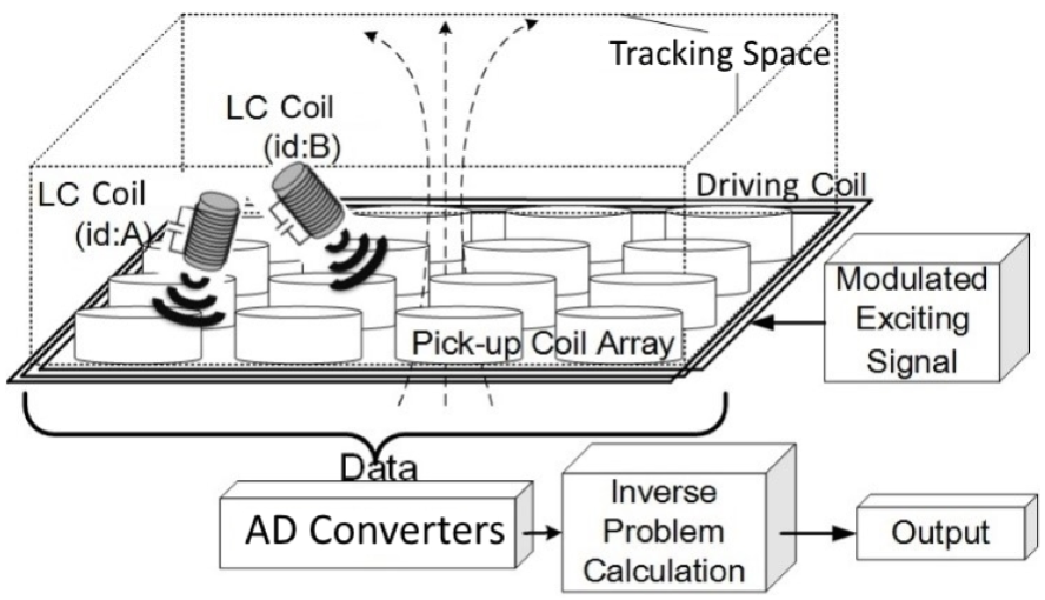
\includegraphics[width=.90\linewidth]{Figures/3 State of the Art/im3d.png}
        \caption{IM3D System Architecture \cite{im3d}}
        \label{fig:im3d-architecture}
    \end{subfigure}%
    \begin{subfigure}{0.40\textwidth}
        \centering
        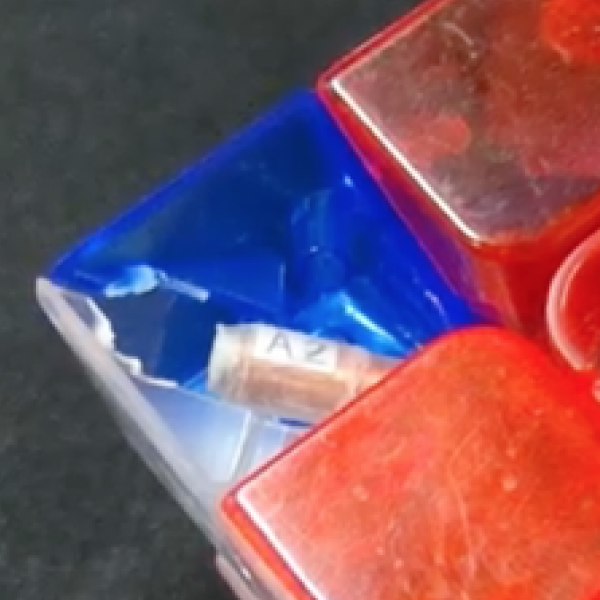
\includegraphics[width=.90\linewidth]{Figures/3 State of the Art/cubeharmonic-2019-tags.png}
        \caption{IM3D trackers in a Rubik's Cube \cite{mannone-cubeharmonic-2019}}
        \label{fig:cubeharmonic-trackers}
    \end{subfigure}%
    \caption{The IM3D technology as used in the Cube Harmonic}
    \label{fig:cubeharmonic-im3d}
\end{figure}

\subsection{Muscle-Tracking Armband}
In 2017, Richard Polfreman and Benjamin Oliver researched ways to use the face turns of a Rubik's Cube as controls for a music synthesizer. They explored the use of a muscle-tracking armband (specifically the Myo Armband) to track the human solver's finger movements while manipulating the cube. However, since "the Myo moved a little when 'cubing'", they ultimately found greater success with a computer vision based tracking solution similar to those discussed in \ref{subsec:computer-vision}.


\section{Other Relevant Research}
Finally, there are a number of research papers/commerical products that seek to transmit data in highly-constrained environments that are potentially relevant to the challenge of tracking the turns of a Rubik's Cube.

This section discusses some of these potential alternate move tracking mediums, specifically sound, RFID, and off-angle magnetic rotation sensors.

\subsection{Sound}
TODO discuss the viability of using sound for making a smart cube.

\subsubsection{Google's "Data Over Sound" Project}
TODO discuss the Google's "data over sound" project and its applicability to this problem space.

\subsection{RFID}
TODO discuss the viability of using RFID for making a smart cube.

\subsection{Off-Angle Magnetic Rotational Sensors}
TODO discuss the viability of using Off-Angle Magnetic Rotational Sensors for making a smart cube.


\section{Choice of Sound for My Thesis}

TODO This section might be large enough to merit its own chapter...
TODO Briefly detail the rationale for chosing to pursue a sound-based approach.